\newpage

\section{Appendix - Alternatives}
\label{sec:dp-pds-appendix}

\subsection{Individual Ground Grids}
\label{sec:dp-pds-appendix-grid}

In collaboration with the \dword{hv} consortium, the installation of individual ground grids for each \dword{pmt} in place of the ground grid table structure is under consideration. Since the individual ground grid cages will potentially have thinner wires and will be closer to the \dword{pmt} windows, generating a smaller shadow, they should increase the acceptance of the \dwords{pmt}.

The feasibility of the design in operation under \dune \dual conditions will be studied by the \dword{hv} consortium. The design of the individual grids will be developed as a common effort of the two consortia engineering teams. The \dword{hv} consortium will produce the grids. The grids will be installed at the \dword{ctsf} by \dual \dword{pd} consortium. The \dwords{pmt} will be installed with their individual grid cages by \dual \dword{pd} consortium. 

\subsection{Calibration System Alternatives}
\label{sec:dp-pds-appendix-calibration}

Alternatives to the baseline design of the calibration system described in Section~\ref{sec:dp-pds-calibration} will be pursued with R\&D measurements to make the system more effective, reduce the cost, and mitigate issues related to scaling to the \dune \dual size. These alternatives include reducing the number of fibers, studying other options for the reference sensor, and increasing the input light if necessary. To reduce the number of fibers, light diffusers can be used, so that one fiber can illuminate at least four \dwords{pmt}. For instance, a diffuser could be placed at the ground grid, or in the case of individual ground grids, on the side walls. With the same aim of reducing the total number of fibers, an alternative calibration system with two fibers placed at the top of the field cage is being tested in \dword{pddp}, so that one fiber can illuminate several \dwords{pmt}. Other than the diffusers and fiber placement, considered alternatives are related to the external system and can be implemented with minimal interference with other subsystems.

\subsection{Xe Doping of Liquid Argon}
\label{sec:dp-pds-appendix-xedoping}

Doping the \dword{lar} volume with Xe is an attractive option in terms of providing a volume distributed wavelength shifting. Major advantages of Xe doping are triggering the long-lived triplet argon excimer to produce a faster signal reducing the fraction of late light; shifting the scintillation signal to longer wavelengths (\SI{175}{nm}) and as a consequence, a longer Rayleigh scattering length.

Dedicated simulations on light yield in the full \dword{dp} \dword{fd} cryostat in the presence of Xe doping were performed. Figure~\ref{fig:dppd_fd_light_yield_xedoping} shows the 1D light yields as a function of the drift (transverse) direction in the left (right) panel, averaging over the other two spatial coordinates. It is evident that the Xe doping can be considered as an immediate alternative to the baseline design with half coverage reflector/\dword{wls} panels in terms of light output. On the other hand, keeping a smaller area coverage reflector/\dword{wls} panels closer to the charge readout may be preferable in order to improve the uniformity.

%\subsection{Wavelength Shifting Reflective Foils}
%\label{sec:dp-pds-appendix-wlsfoils}

%To enhance light collection and improve response uniformity in the detector volume, installing wavelength shifting reflector foils on the \dword{fc} inner surfaces is under consideration. This alternative is being evaluated for two particular cases: covering \dword{fc} inner walls fully with the foils and covering only the upper half of the \dword{fc} with the foils. In addition to completely evaluating the effect on physics within the consortium, the interface, particularly the effect on liquid circulation, the effective electric field, and the mechanical structure are being discussed with the \dword{hv} consortium.

%\fixme{If included in the baseline design, move to section \ref{sec:dp-pds-mechanics}}

\begin{dunefigure}[Expected 1D light yields in the full \dword{dp} \dword{fd} cryostat, with xenon doping.]{fig:dppd_fd_light_yield_xedoping}
{Expected light yield in the full \dword{dp} \dword{fd} cryostat in the presence of xenon doping. The yield units are number of photo-electrons per \si{\MeV} of deposited energy. The 1D yields are shown as a function of the drift (transverse) direction in the left (right) panel, averaging over the other two spatial coordinates (not shown), similarly to Fig.~\ref{fig:dppd_fd_light_yield_comparisons}. The three histograms correspond to the half foil baseline design without xenon doping, and to two no foil geometries, with and without xenon doping, respectively.}
\raisebox{0.1cm}{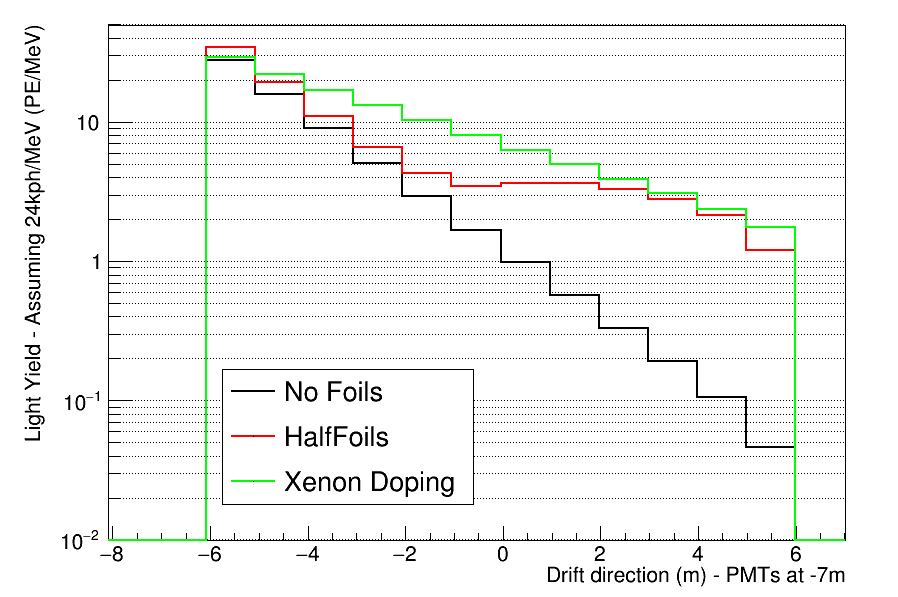
\includegraphics[width=0.49\textwidth]{graphics/dppd_xedoping_drift.png}} \hfill
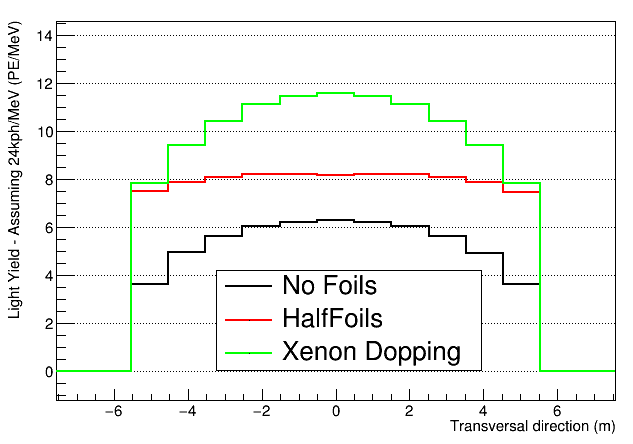
\includegraphics[width=0.49\textwidth]{graphics/dppd_xedoping_transverse.png}
\end{dunefigure}